
\section{Background}
\label{ref:background}
\begin{figure*}
\begin{center}
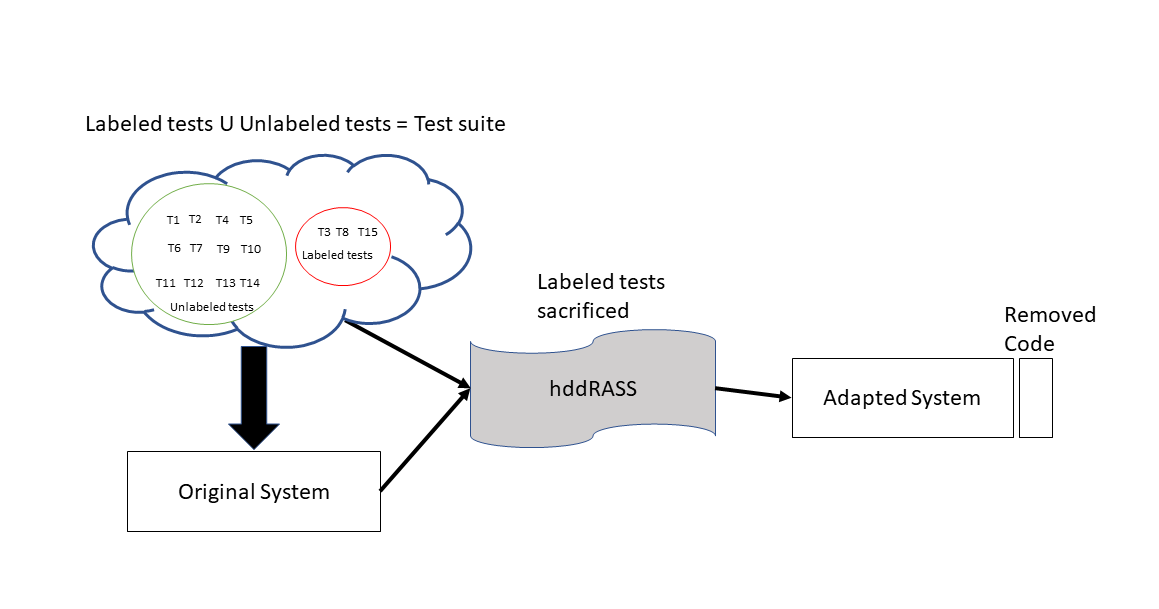
\includegraphics[scale = 0.50]{icst_19_fig1.png}
\caption{TBSM approach to build adaptation for single adaptation objective
scenario. Labeled tests encode adaptation specification for single resource
variability.}
\label{fig:workflow}
\end{center}
\end{figure*}

While working with developers attempting to build SAS for a real-world, mission-critical system, we observed that (1) most developers speak the language of tests fluently, unlike that of formal methods or architectural descriptions,  (2) tests are thus, for even most complex projects in the real world, the \emph{only} semi-formal specification available. To exploit both the widespread availability of tests for mission-critical systems and developers' familiarity with tests, we proposed capturing resource adaptation specifications using tests.
TBSM relies on developers' understanding of tests, and how tests relate to program features and resource usage. Developers encode this information by simply labeling the tests. Test labels can be a multi-dimensional space in feature, resource, and priority. To demonstrate the concept, we assume a single adaptation objective: a single resource faces variability or unavailibility. The concept is demonstrated in Fig.~\ref{fig:workflow} (a simplified version of Fig 2. in the original paper proposing TBSM~\cite{christi2017saso}. We reuse this figure from our previous work to keep the paper self-contained.~\cite{christi2019qrs}). Labeled tests define functionality that can be sacrificed to reduce resource usage. Unlabeled tests define the functionality that is to be retained and not modified. A tool called hddRASS takes as its input the test suite with labeled and unlabeled tests and the original program, and produces a minimized program such that the functionality marked by labeled tests is removed. hddRASS achieves this by temporarily removing the labeled tests from the suite and using the Hierarchical Delta Debugging (HDD) algorithm to find a minimal program, such that retained tests continue to pass~\cite{misherghi2006hdd}. The basic idea is that if the labeled tests define a functionality that uses resources, removing that functionality will ensure resource adaptation. TBSM builds adaptations, in a sense, in the same way that Automatic Program Repair fixes faults. In APR, the goal is to modify the program to pass a set of previously failing tests (without failing previously passing tests)~\cite{monperrus2018asr}. In TBSM, the goal is to modify the program while removing as much code as possible, while still passing a set of unlabeled tests.

